\providecommand{\Fun}{\operatorname{Fun}}
\providecommand{\Cat}{\mathcal{C}at}
\providecommand{\QCat}{\mathcal{Q}\mathcal{C}at}
\providecommand{\sSet}{s\mathcal{S}et}
\providecommand{\qcOne}{\mathbf{1}}   %
\providecommand{\colim}{\operatorname{colim}\nolimits}

\section{\trLimit{}与\trColimit{}的保持}\label{sec:preservation-of-limits-and-colimits}

\trFunctor $f\colon A\to B$ \emph{保持\trLimit}（preserves limits），
如果 $A$ 中某个\trLimit\trCone{}在 $f$ 下的像也在 $B$ 中定义一个%
\trLimit\trCone。反方向地，\trFunctor $f\colon A\to B$ \emph{反射\trLimit}%
（reflects limits），如果 $A$ 中某个\trCone——其在 $f$ 下的像于 $B$ 中定义
一个\trLimit\trCone——本身也是 $A$ 中的\trLimit\trCone。而\trFunctor
$f\colon A\to B$ \emph{创建\trLimit}（creates limits），如果只要 $A$ 中的
一个\trDiagram{}在 $B$ 中拥有\trLimit\trCone，$A$ 中就必然存在一个%
\trLimit\trCone，其经 $f$ 的像与 $B$ 中给定的那个\trLimit\trCone{}同构。

著名的事实是：\trRightAdjoint{}保持\trLimit，\trLeftAdjoint{}保持\trColimit。
本节的目标便是在\trInfinityCategory{}的语境中证明这一点，并展示始函子与
终函子（initial and final functors，含义见\cref{def:initial-final-functors}）
最初的几个例子。我们以一个关于\trLimit{}反射的结果作结，其证明关键性地
依赖一条结果——\trCosmologicalFunctor{}保持绝对\trLifting{}图——正是它引出了第 3 章。

\trRightAdjoint{}与\trLimit{}之间的可交换性，在所论\trInfinityCategory{}%
具有某种给定形状的\emph{全部}\trLimit{}的情形中，是极易建立的：在这些
假设下，\trLimit\trFunctor{}是\trConstantFunctor{}的\trRightAdjoint，
而\trConstantFunctor{}与基\trInfinityCategory{}之间的任何\trFunctor{}都
可交换。由于诸\trLeftAdjoint{}可交换，\trAdjunction{}的唯一性
（\cref{prop:uniqueness-of-adjoints}）便蕴含：诸\trRightAdjoint{}在
同构意义下可交换。这一概要为\cref{ex:preservation-commuting-squares}
提供了提示。

在一般情形需要更精细的论证——比如，在不预先假设任何其他\trLimit{}存在
的情况下保持单个\trLimit\trDiagram。我们诉诸一条关于绝对\trLifting{}图
之合成与消去的一般引理：

\begin{lemma}[绝对\trLifting{}图的合成与消去]\label{lem:composition-cancelation-lifting}
设 $(r,\rho)$ 定义了 $h$ 沿 $f$ 的一个绝对右\trLifting：
\begin{center}
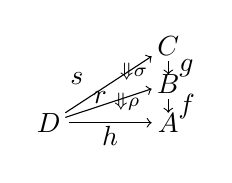
\begin{tikzpicture}[x=1.2em,y=1.2em]
  \node (D1) at (0,0) {$D$};
  \node (C1) at (3.6,2.3) {$C$};
  \node (B1) at (3.6,1.15) {$B$};
  \node (A1) at (3.6,0) {$A$};
  \draw[->] (0.5,0.3) -- (3.1,2.0);
  \node at (0.85,1.32) {$s$};
  \draw[->] (3.6,1.85) -- (3.6,1.45);
  \node at (4.15,1.65) {$g$};
  \draw[->] (3.6,0.7) -- (3.6,0.3);
  \node at (4.15,0.5) {$f$};
  \draw[->] (0.5,0.16) -- (3.1,1.02);
  \node at (1.55,0.75) {$r$};
  \draw[->] (0.6,0) -- (3.1,0);
  \node at (1.85,-0.4) {$h$};
  \node at (2.55,1.55) {$\scriptstyle\Downarrow\sigma$};
  \node at (2.35,0.62) {$\scriptstyle\Downarrow\rho$};
\end{tikzpicture}
\end{center}
那么 $(s,\sigma)$ 定义了 $r$ 沿 $g$ 的一个绝对右\trLifting，当且仅当
$(s,\rho\cdot f\sigma)$ 定义了 $h$ 沿 $fg$ 的一个绝对右\trLifting。
\end{lemma}

\begin{proof}
\cref{lem:composition-cancelation-lifting}的证明是%
\cref{ex:prove-lemma-composition}。
\end{proof}

\begin{theorem}\label{thm:right-adjoints-preserve-limits}
\trRightAdjoint{}保持\trLimit，而\trLeftAdjoint{}保持\trColimit。
\end{theorem}

\trRightAdjoint{}保持\trLimit{}的标准论证是这样的：\trRightAdjoint $u$
的像中某个 $J$ 形状\trDiagram{}上的一个\trCone，跨\trAdjunction
$f^{J}\dashv u^{J}$ 转置为原\trDiagram{}上的一个\trCone，后者经由指定的%
\trLimit\trCone{}唯一分解。这一分解再跨\trAdjunction $f\dashv u$ 转置，
便定义出所要的、经由\trLimit\trCone{}之像的唯一分解。沿这条路线也同样
可以给出一个\trInfinityCategory{}式的证明（见\cref{ex:gap-in-bogus-proof}），
但我们改而呈示标准论证的一个更利落的封装：我们用绝对\trLifting{}图
来表达\trLimit{}与\trColimit{}的泛性质（\cref{def:limit-colimit-cones}）
与伴随转置（\cref{lem:unit-counit-absolute-liftings}），从而无须考虑一个
必须被证明唯一地经由\trLimit\trCone{}分解的一般检验\trCone。

\begin{proof}
我们证明\trRightAdjoint{}保持\trLimit。取余对偶，同一论证便证明%
\trLeftAdjoint{}保持\trColimit。

设\trInfinityCosmos $\mathcal{K}$ 中的\trFunctor $u\colon A\to B$ 容许一个
带\trCounit $\epsilon\colon fu\Rightarrow\mathrm{id}_A$ 的\trLeftAdjoint
$f\colon B\to A$。我们的目标是证明：任何如下左图所示的绝对右\trLifting{}图，
都被携带为如下右图所示的绝对右\trLifting{}图：
\begin{rveq}\label{eq:adjoint-commutes-limits}
\mbox{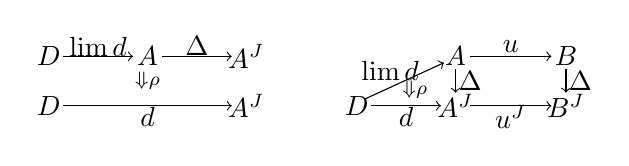
\begin{tikzpicture}[x=1.05em,y=1.05em]
  \node (D1) at (0,0) {$D$};
  \node (Am) at (3.4,0) {$A$};
  \node (AJ1) at (6.8,0) {$A^{J}$};
  \draw[->] (0.5,0) -- (2.9,0);
  \node at (1.7,0.34) {$\lim d$};
  \draw[->] (3.9,0) -- (6.3,0);
  \node at (5.1,0.34) {$\Delta$};
  \node (D2) at (0,-1.7) {$D$};
  \node (AJ2) at (6.8,-1.7) {$A^{J}$};
  \draw[->] (0.5,-1.7) -- (6.3,-1.7);
  \node at (3.4,-2.08) {$d$};
  \node at (3.4,-0.85) {$\scriptstyle\Downarrow\rho$};
  \node (D3) at (10.6,-1.7) {$D$};
  \node (A3) at (14.0,0) {$A$};
  \node (B3) at (17.8,0) {$B$};
  \node (AJ3) at (14.0,-1.7) {$A^{J}$};
  \node (BJ3) at (17.8,-1.7) {$B^{J}$};
  \draw[->] (10.85,-1.48) -- (13.6,-0.22);
  \node at (11.75,-0.5) {$\lim d$};
  \node at (12.6,-1.15) {$\scriptstyle\Downarrow\rho$};
  \draw[->] (14.5,0) -- (17.3,0);
  \node at (15.9,0.34) {$u$};
  \draw[->] (14.0,-0.45) -- (14.0,-1.25);
  \node at (14.5,-0.85) {$\Delta$};
  \draw[->] (17.8,-0.45) -- (17.8,-1.25);
  \node at (18.3,-0.85) {$\Delta$};
  \draw[->] (11.1,-1.7) -- (13.5,-1.7);
  \node at (12.3,-2.08) {$d$};
  \draw[->] (14.5,-1.7) -- (17.3,-1.7);
  \node at (15.9,-2.08) {$u^{J}$};
\end{tikzpicture}}
\end{rveq}
由\cref{prop:adjunction-preservation}，\trSimplicial\trCotensor
$(-)^{J}\colon\mathrm{h}\mathcal{K}\to\mathrm{h}\mathcal{K}$ 把\trAdjunction
$f\dashv u$ 携带为带\trCounit $\epsilon^{J}$ 的\trAdjunction
$f^{J}\dashv u^{J}$。特别地，由\cref{lem:unit-counit-absolute-liftings}，
$(u^{J},\epsilon^{J})$ 定义了恒同沿 $f^{J}$ 的一个绝对右\trLifting，
而后者在沿\trFunctor $d$ 的限制下保持。于是，由%
\cref{lem:composition-cancelation-lifting}，%
\cref{eq:adjoint-commutes-limits}右图的图是绝对右\trLifting{}图，当且仅当
下左图所示的粘贴复合定义一张绝对右\trLifting{}图：
\begin{center}
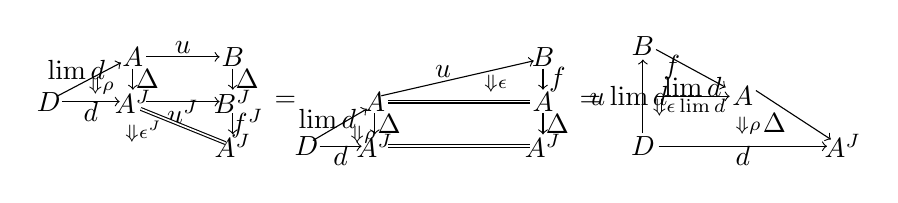
\begin{tikzpicture}[x=0.95em,y=0.95em]
  \node (L1D) at (0,-1.7) {$D$};
  \node (L1A) at (3.2,0) {$A$};
  \node (L1B) at (7.0,0) {$B$};
  \node (L1AJ1) at (3.2,-1.7) {$A^{J}$};
  \node (L1BJ) at (7.0,-1.7) {$B^{J}$};
  \node (L1AJ2) at (7.0,-3.4) {$A^{J}$};
  \draw[->] (0.35,-1.48) -- (2.75,-0.22);
  \node at (1.05,-0.5) {$\lim d$};
  \node at (2.0,-1.1) {$\scriptstyle\Downarrow\rho$};
  \draw[->] (3.7,0) -- (6.5,0);
  \node at (5.1,0.34) {$u$};
  \draw[->] (3.2,-0.45) -- (3.2,-1.25);
  \node at (3.75,-0.85) {$\Delta$};
  \draw[->] (7.0,-0.45) -- (7.0,-1.25);
  \node at (7.55,-0.85) {$\Delta$};
  \draw[->] (0.5,-1.7) -- (2.7,-1.7);
  \node at (1.6,-2.08) {$d$};
  \draw[->] (3.7,-1.7) -- (6.5,-1.7);
  \node at (5.1,-2.08) {$u^{J}$};
  \draw[double] (3.5,-1.98) -- (6.72,-3.28);
  \node at (3.6,-2.85) {$\scriptstyle\Downarrow\epsilon^{J}$};
  \draw[->] (7.0,-2.15) -- (7.0,-2.95);
  \node at (7.55,-2.55) {$f^{J}$};
  \node at (9.0,-1.7) {$=$};
  \node (M1D) at (9.8,-3.4) {$D$};
  \node (M1A1) at (12.4,-1.7) {$A$};
  \node (M1A2) at (18.8,-1.7) {$A$};
  \node (M1B) at (18.8,0) {$B$};
  \node (M1AJ1) at (12.4,-3.4) {$A^{J}$};
  \node (M1AJ2) at (18.8,-3.4) {$A^{J}$};
  \draw[->] (12.65,-1.48) -- (18.45,-0.15);
  \node at (15.0,-0.55) {$u$};
  \node at (17.0,-1.0) {$\scriptstyle\Downarrow\epsilon$};
  \draw[->] (18.8,-0.45) -- (18.8,-1.25);
  \node at (19.35,-0.85) {$f$};
  \draw[double] (12.9,-1.7) -- (18.3,-1.7);
  \draw[->] (12.4,-2.15) -- (12.4,-2.95);
  \node at (12.95,-2.55) {$\Delta$};
  \draw[->] (18.8,-2.15) -- (18.8,-2.95);
  \node at (19.35,-2.55) {$\Delta$};
  \draw[->] (10.05,-3.18) -- (12.1,-1.98);
  \node at (10.6,-2.35) {$\lim d$};
  \node at (11.95,-2.95) {$\scriptstyle\Downarrow\rho$};
  \draw[->] (10.3,-3.4) -- (11.9,-3.4);
  \node at (11.1,-3.78) {$d$};
  \draw[double] (12.9,-3.4) -- (18.3,-3.4);
  \node at (20.6,-1.7) {$=$};
  \node (RD) at (22.6,-3.4) {$D$};
  \node (RB) at (22.6,0.4) {$B$};
  \node (RA) at (26.4,-1.5) {$A$};
  \node (RAJ) at (30.2,-3.4) {$A^{J}$};
  \draw[->] (22.6,-2.9) -- (22.6,-0.1);
  \node at (22.05,-1.5) {$u\lim d$};
  \draw[->] (23.1,0.28) -- (25.75,-1.16);
  \node at (23.7,-0.4) {$f$};
  \draw[->] (23.1,-1.5) -- (25.9,-1.5);
  \node at (24.5,-1.14) {$\lim d$};
  \draw[->] (26.9,-1.28) -- (29.75,-3.14);
  \node at (27.6,-2.5) {$\Delta$};
  \draw[->] (23.2,-3.4) -- (29.6,-3.4);
  \node at (26.4,-3.78) {$d$};
  \node at (24.35,-1.95) {$\scriptstyle\Downarrow\epsilon\lim d$};
  \node at (26.6,-2.62) {$\scriptstyle\Downarrow\rho$};
\end{tikzpicture}
\end{center}
如\cref{lem:unit-counit-absolute-liftings}的证明中所注记的，把%
\cref{eq:adjoint-commutes-limits}右侧的 2-\trCell{}与\trCounit{}按这种方式
粘贴，相当于把\trCone $u^{J}\rho$ 跨\trAdjunction $f^{J}\dashv u^{J}$
作转置。

我们现在论证：上左这张转置后的\trCone{}以一种典范的方式经由\trLimit\trCone
$(\lim d,\rho)$ 分解。由单纯\trCotensor{}关于其指数变元的\trTwoFunctor{}性，
$f^{J}\Delta=\Delta f$ 且 $\epsilon^{J}\Delta=\Delta\epsilon$。因此，上左
所示的粘贴图等于上中所示的图，后者又等于上右的图。最后的这张图是两张绝对
右\trLifting{}图的粘贴复合，从而由\cref{lem:composition-cancelation-lifting}，
其自身也是一张绝对右\trLifting{}图；这一\trUniversalProperty{}是说：任何
顶点经 $f$ 分解的 $d$ 上的\trCone，都唯一地经由\trLimit\trCone
$(\lim d,\rho)$ 分解——分解所用的映射继而又跨\trAdjunction $f\dashv u$
转置。于是，\cref{eq:adjoint-commutes-limits}右端的图如所断言，是一张绝对
右\trLifting{}图。
\end{proof}

\begin{proposition}\label{prop:equivalences-limits}
\trInfinityCategory{}之间的一个\trEquivalence $f\colon A\simeq B$ 保持、
反射并创建\trLimit{}与\trColimit。
\end{proposition}

\begin{proof}
由\cref{prop:adjoint-equivalences}，\trEquivalence{}定义出伴随\trFunctor，
故\cref{thm:right-adjoints-preserve-limits}蕴含：\trEquivalence{}保持%
\trLimit。为看出\trLimit{}被反射，考虑 $A$ 中一个 $J$ 形状的\trCone
$\rho$，设其像 $f^{J}\rho$ 是 $B$ 中的一个\trLimit\trCone。逆\trEquivalence
$g\colon B\rightleftarrows A$ 把它携带为 $A$ 中的一个\trLimit\trCone
$gf^{J}\rho$，后者与原先的\trCone $\rho$ 自然同构。由\cref{ex:lifting-invariance-under-iso}，
$\rho$ 必定也定义一个\trLimit\trCone。
最后，为看出\trLimit{}被创建，考虑\trDiagram $d\colon D\to A^J$，设 $fd$
在 $B$ 中拥有一个\trLimit\trCone $\nu$。于是 $g^{J}\nu$ 为\trDiagram
$gfd$ 在 $A$ 中定义一个\trLimit\trCone，而由\cref{ex:lifting-invariance-under-iso}，$d$ 的一个%
\trLimit\trCone{}可通过与同构 $gfd\cong d$ 复合而定义。
\end{proof}

我们现在转向另一类\trLimit{}保持结果，它可用来简化具有特定形状的%
\trDiagram{}之\trLimit{}或\trColimit{}的计算。这一简化是这样实现的：
沿一个\trFunctor $k\colon I\to J$ 作限制，从而对\trDiagram{}重新索引。
对某些\trFunctor——称作「始的」与「终的」——这种重索引分别保持并反射%
\trLimit{}或\trColimit。

眼下我们给出这些\trFunctor{}的一种目的论式的、而非内在的刻画。下面的
定义对\trCartesianClosed{}\trInfinityCosmos{}中的任意\trFunctor{}有意义，
也对在任意\trInfinityCosmos{}中充当索引形状的\trSimplicialSet{}之间的
映射有意义。在定义 9.4.11 中，我们把形容词「始的」与「终的」扩充到任意%
\trInfinityCosmos{}中\trInfinityCategory{}之间的\trFunctor{}上，并证明
在那里得到刻画的\trFunctor{}满足此处所述的性质。

\begin{definition}[始函子与终函子]\label{def:initial-final-functors}
\trFunctor $k\colon I\to J$ 是\textbf{终函子}（final functor），如果
$J$ 形状的\trCone{}定义一个\trColimit\trCone，当且仅当限制所得的
$I$ 形状\trCone{}是\trColimit\trCone；$k$ 是\textbf{始函子}（initial
functor），如果 $J$ 形状的\trCone{}定义一个\trLimit\trCone，
当且仅当限制所得的 $I$ 形状\trCone{}是\trLimit\trCone。也就是说，
$k\colon I\to J$ 是终函子，当且仅当对任何\trInfinityCategory $A$，方块
\begin{center}
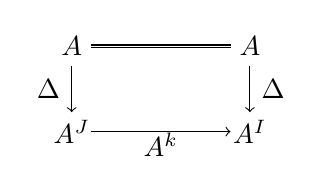
\begin{tikzpicture}[x=1.4em,y=1.4em]
  \node (AL) at (0,0) {$A$};
  \node (AR) at (4.6,0) {$A$};
  \node (J) at (0,-2.2) {$A^{J}$};
  \node (I) at (4.6,-2.2) {$A^{I}$};
  \draw[double] (0.5,0) -- (4.1,0);
  \draw[->] (0,-0.5) -- (0,-1.7);
  \node at (-0.6,-1.1) {$\Delta$};
  \draw[->] (4.6,-0.5) -- (4.6,-1.7);
  \node at (5.2,-1.1) {$\Delta$};
  \draw[->] (0.5,-2.2) -- (4.1,-2.2);
  \node at (2.3,-2.54) {$A^{k}$};
\end{tikzpicture}
\end{center}
保持并反射一切绝对左\trLifting{}图；$k$ 是始函子，当且仅当该方块保持
并反射一切绝对右\trLifting{}图。
\end{definition}

历史上，终函子曾被称为「余终函子」（cofinal），而对偶概念则没有显而易见
的名称。我们偏爱的术语系于如下的记忆法：\trInitial{}元素的包含定义一个
始函子，而\trTerminal{}元素（terminal，又称 final 元素）的包含定义一个
终函子。这些事实是一个更一般结果的特例；我们现在就来建立这个结果，所用
的策略与\cref{thm:right-adjoints-preserve-limits}的证明中所部署者
完全相同。

\begin{proposition}\label{prop:left-adjoints-initial}
\trLeftAdjoint{}定义始函子，而\trRightAdjoint{}定义终函子。
\end{proposition}

\begin{proof}
设 $k\dashv r$ 带\trCounit $\epsilon\colon kr\Rightarrow\mathrm{id}_J$，
则对 $A$ 作\trCotensor{}便得到一个\trAdjunction
\begin{center}
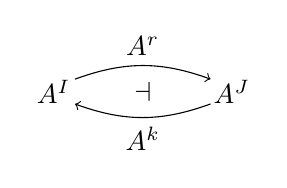
\begin{tikzpicture}[x=1.4em,y=1.4em]
  \node (AI) at (0,0) {$A^{I}$};
  \node (AJ) at (4.6,0) {$A^{J}$};
  \draw[->] (0.55,0.32) to[bend left=20] node[above]{$A^{r}$} (4.05,0.32);
  \node at (2.3,0) {$\dashv$};
  \draw[->] (4.05,-0.32) to[bend left=20] node[below]{$A^{k}$} (0.55,-0.32);
\end{tikzpicture}
\end{center}
其\trCounit{}为 $A^{\epsilon}\colon A^{r}A^{k}\Rightarrow\mathrm{id}_{A^{J}}$。
为证明 $k$ 是始函子，我们必须证明：对如下左图所示的任意\trCone
$\rho\colon\Delta\ell\Rightarrow d$，
\begin{center}
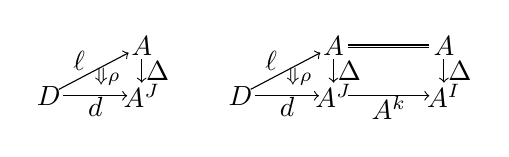
\begin{tikzpicture}[x=1.05em,y=1.05em]
  \node (L1D) at (0,-1.7) {$D$};
  \node (L1A) at (3.2,0) {$A$};
  \node (L1AJ) at (3.2,-1.7) {$A^{J}$};
  \draw[->] (0.35,-1.48) -- (2.75,-0.22);
  \node at (1.05,-0.5) {$\ell$};
  \node at (2.0,-1.05) {$\scriptstyle\Downarrow\rho$};
  \draw[->] (3.2,-0.45) -- (3.2,-1.25);
  \node at (3.75,-0.85) {$\Delta$};
  \draw[->] (0.5,-1.7) -- (2.7,-1.7);
  \node at (1.6,-2.08) {$d$};
  \node (R1D) at (6.6,-1.7) {$D$};
  \node (R1A1) at (9.8,0) {$A$};
  \node (R1A2) at (13.6,0) {$A$};
  \node (R1AJ) at (9.8,-1.7) {$A^{J}$};
  \node (R1AI) at (13.6,-1.7) {$A^{I}$};
  \draw[double] (10.3,0) -- (13.1,0);
  \draw[->] (6.95,-1.48) -- (9.35,-0.22);
  \node at (7.65,-0.5) {$\ell$};
  \node at (8.6,-1.05) {$\scriptstyle\Downarrow\rho$};
  \draw[->] (9.8,-0.45) -- (9.8,-1.25);
  \node at (10.35,-0.85) {$\Delta$};
  \draw[->] (13.6,-0.45) -- (13.6,-1.25);
  \node at (14.15,-0.85) {$\Delta$};
  \draw[->] (7.1,-1.7) -- (9.3,-1.7);
  \node at (8.2,-2.08) {$d$};
  \draw[->] (10.3,-1.7) -- (13.1,-1.7);
  \node at (11.7,-2.1) {$A^{k}$};
\end{tikzpicture}
\end{center}
左图是一张绝对右\trLifting{}图，当且仅当右图是一张绝对右\trLifting{}图。
由\cref{lem:unit-counit-absolute-liftings}与\cref{lem:composition-cancelation-lifting}，
右图是一张绝对右\trLifting{}图，当且仅当下左图所示的粘贴复合也是一张绝对
右\trLifting{}图：
\begin{center}
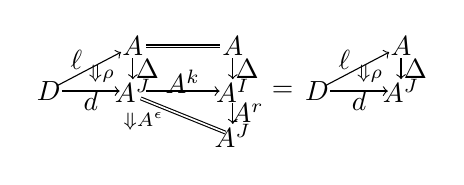
\begin{tikzpicture}[x=0.95em,y=0.95em]
  \node (P1D) at (0,-1.7) {$D$};
  \node (P1A1) at (3.2,0) {$A$};
  \node (P1A2) at (7.0,0) {$A$};
  \node (P1AJ) at (3.2,-1.7) {$A^{J}$};
  \node (P1AI) at (7.0,-1.7) {$A^{I}$};
  \node (P1AJ2) at (7.0,-3.4) {$A^{J}$};
  \draw[double] (3.7,0) -- (6.5,0);
  \draw[->] (0.35,-1.48) -- (2.75,-0.22);
  \node at (1.05,-0.5) {$\ell$};
  \node at (2.0,-1.05) {$\scriptstyle\Downarrow\rho$};
  \draw[->] (3.2,-0.45) -- (3.2,-1.25);
  \node at (3.75,-0.85) {$\Delta$};
  \draw[->] (7.0,-0.45) -- (7.0,-1.25);
  \node at (7.55,-0.85) {$\Delta$};
  \draw[->] (0.5,-1.7) -- (2.7,-1.7);
  \node at (1.6,-2.08) {$d$};
  \draw[->] (3.7,-1.7) -- (6.5,-1.7);
  \node at (5.1,-1.36) {$A^{k}$};
  \draw[double] (3.5,-1.98) -- (6.72,-3.28);
  \node at (3.6,-2.85) {$\scriptstyle\Downarrow A^{\epsilon}$};
  \draw[->] (7.0,-2.15) -- (7.0,-2.95);
  \node at (7.55,-2.55) {$A^{r}$};
  \node at (8.9,-1.7) {$=$};
  \node (Q1D) at (10.2,-1.7) {$D$};
  \node (Q1A) at (13.4,0) {$A$};
  \node (Q1AJ) at (13.4,-1.7) {$A^{J}$};
  \draw[->] (10.55,-1.48) -- (12.95,-0.22);
  \node at (11.25,-0.5) {$\ell$};
  \node at (12.2,-1.05) {$\scriptstyle\Downarrow\rho$};
  \draw[->] (13.4,-0.45) -- (13.4,-1.25);
  \node at (13.95,-0.85) {$\Delta$};
  \draw[->] (10.7,-1.7) -- (12.9,-1.7);
  \node at (11.8,-2.08) {$d$};
\end{tikzpicture}
\end{center}
由于 $A^{r}\Delta=\Delta$ 且 $A^{\epsilon}\Delta=\mathrm{id}_{\Delta}$，
左端化归为右端，这就证明了断言。
\end{proof}

\cref{ex:fully-faithful-liftings}把\trInfinityCategory{}之间的一个\trFunctor $f\colon A\to B$
定义为\textbf{\trFullyFaithful}（fully faithful），当且仅当下图
\begin{center}
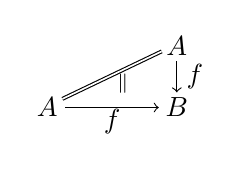
\begin{tikzpicture}[x=1.3em,y=1.3em]
  \node (A1) at (0,0) {$A$};
  \node (A2) at (3.6,1.7) {$A$};
  \node (B2) at (3.6,0) {$B$};
  \draw[double] (0.42,0.24) -- (3.18,1.56);
  \draw[->] (3.6,1.28) -- (3.6,0.42);
  \node at (4.1,0.85) {$f$};
  \draw[->] (0.5,0) -- (3.1,0);
  \node at (1.8,-0.4) {$f$};
  \node at (2.1,0.66) {$\scriptstyle\Vert$};
\end{tikzpicture}
\end{center}
定义一张绝对右\trLifting{}图，或等价地，定义一张绝对左\trLifting{}图。
除一条我们从第 3 章借来的结果外，我们将证明：

\begin{proposition}[全忠实\trFunctor{}反射\trLimit]\label{prop:fully-faithful-reflect-limits}
一个全忠实的\trFunctor $f\colon A\to B$ 反射 $B$ 中存在的一切\trLimit{}%
或\trColimit。
\end{proposition}

\begin{proof}
关于\trLimit{}的断言是说：对 $A$ 中形状 $J$ 的任何\trDiagram{}族
$d\colon D\to A^{J}$、任何\trFunctor $\ell\colon D\to A$ 以及任何\trCone
$\rho\colon\Delta\ell\Rightarrow d$，只要它与 $f^{J}\colon A^{J}\to B^{J}$
的\trWhiskering{}是如下一张绝对右\trLifting{}图
\begin{center}
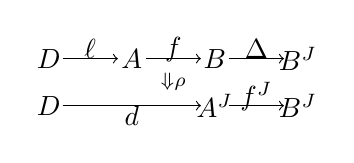
\begin{tikzpicture}[x=1.0em,y=1.0em]
  \node (D1) at (0,0) {$D$};
  \node (A1) at (3.0,0) {$A$};
  \node (B1) at (6.0,0) {$B$};
  \node (BJ1) at (9.0,0) {$B^{J}$};
  \draw[->] (0.5,0) -- (2.5,0);
  \node at (1.5,0.34) {$\ell$};
  \draw[->] (3.5,0) -- (5.5,0);
  \node at (4.5,0.34) {$f$};
  \draw[->] (6.5,0) -- (8.5,0);
  \node at (7.5,0.34) {$\Delta$};
  \node (D2) at (0,-1.7) {$D$};
  \node (AJ2) at (6.0,-1.7) {$A^{J}$};
  \node (BJ2) at (9.0,-1.7) {$B^{J}$};
  \draw[->] (0.5,-1.7) -- (5.5,-1.7);
  \node at (3.0,-2.08) {$d$};
  \draw[->] (6.5,-1.7) -- (8.5,-1.7);
  \node at (7.5,-1.36) {$f^{J}$};
  \node at (4.5,-0.85) {$\scriptstyle\Downarrow\rho$};
\end{tikzpicture}
\end{center}
那么 $(\ell,\rho)$ 便定义 $d\colon D\to A^{J}$ 沿 $\Delta\colon A\to A^{J}$
的一个绝对右\trLifting。由\cref{ex:fully-faithful-liftings}，说 $f$ 是全忠实的，等于说
$\mathrm{id}_A\colon A\to A$ 定义了 $f$ 沿其自身的一个绝对右\trLifting。
于是由\cref{lem:composition-cancelation-lifting}，下左的复合图是一张绝对
右\trLifting{}图；而由单纯\trCotensor{}关于 $J$ 的\trTwoFunctor{}性，下左
的图与下右的图相重合：
\begin{center}
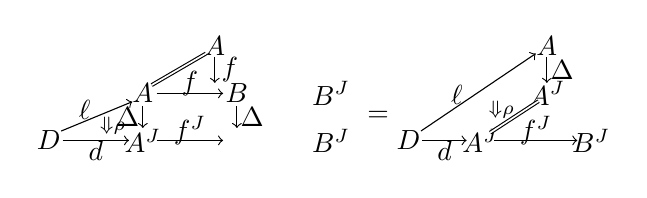
\begin{tikzpicture}[x=1.0em,y=1.0em]
  \node (ALt) at (6.0,1.7) {$A$};
  \node (DL) at (0,-1.7) {$D$};
  \node (AL) at (3.4,0) {$A$};
  \node (BL) at (6.8,0) {$B$};
  \node (BJL) at (10.2,0) {$B^{J}$};
  \node (AJL) at (3.4,-1.7) {$A^{J}$};
  \node (BJL2) at (10.2,-1.7) {$B^{J}$};
  \draw[double] (5.68,1.44) -- (3.72,0.3);      %
  \draw[->] (6.0,1.32) -- (6.0,0.38);           %
  \node at (6.55,0.85) {$f$};
  \draw[->] (0.45,-1.36) -- (3.02,-0.3);        %
  \node at (1.3,-0.6) {$\ell$};
  \draw[->] (3.9,0) -- (6.3,0);                 %
  \node at (5.1,0.34) {$f$};
  \draw[->] (6.8,-0.45) -- (6.8,-1.25);         %
  \node at (7.35,-0.85) {$\Delta$};
  \draw[->] (3.4,-0.45) -- (3.4,-1.25);         %
  \node at (2.85,-0.85) {$\Delta$};
  \draw[->] (0.5,-1.7) -- (2.9,-1.7);           %
  \node at (1.7,-2.08) {$d$};
  \draw[->] (3.9,-1.7) -- (6.3,-1.7);           %
  \node at (5.1,-1.36) {$f^{J}$};
  \node at (2.3,-1.15) {$\scriptstyle\Downarrow\rho$};
  \node at (11.9,-0.85) {$=$};
  \node (ART) at (18.0,1.7) {$A$};
  \node (DR) at (13.0,-1.7) {$D$};
  \node (AJR) at (18.0,0) {$A^{J}$};
  \node (AJR2) at (15.6,-1.7) {$A^{J}$};
  \node (BJR) at (19.6,-1.7) {$B^{J}$};
  \draw[->] (13.45,-1.36) -- (17.6,1.44);       %
  \node at (14.75,-0.05) {$\ell$};
  \draw[->] (18.0,1.32) -- (18.0,0.38);         %
  \node at (18.55,0.85) {$\Delta$};
  \draw[double] (17.7,-0.28) -- (15.95,-1.42);  %
  \node at (16.35,-0.6) {$\scriptstyle\Downarrow\rho$};
  \draw[->] (13.5,-1.7) -- (15.1,-1.7);         %
  \node at (14.3,-2.08) {$d$};
  \draw[->] (16.1,-1.7) -- (19.1,-1.7);         %
  \node at (17.6,-1.36) {$f^{J}$};
\end{tikzpicture}
\end{center}
现在，倘若我们知道 $\mathrm{id}_{A^{J}}\colon A^{J}\to A^{J}$ 定义了
$f^{J}$ 沿其自身的一个绝对右\trLifting——也就是说，倘若我们知道
$f^{J}\colon A^{J}\to B^{J}$ 也是全忠实的——那么再应用一次%
\cref{lem:composition-cancelation-lifting}，便可得出 $(\ell,\rho)$ 是 $d$
沿 $\Delta$ 的一个绝对右\trLifting，一如所需。而事实正是如此：由推论
3.5.7，任何\trCosmologicalFunctor{}——例如 $(-)^{J}$——都保持绝对\trLifting{}图。
\end{proof}

值得问一问：为什么我们还不曾证明\trCosmologicalFunctor{}保持绝对\trLifting{}图？毕竟，
由引理 1.4.4，\trCosmologicalFunctor{}诱导\trHomotopyTwoCategory{}之间的\trTwoFunctor，
而绝对\trLifting{}图正是在那里定义的。但\trAdjunction{}与它们不同：
\trAdjunction{}由 2-\trCategory{}中的粘贴等式定义，而绝对\trLifting{}图
的定义使用了全称量词，因此并非被所有\trTwoFunctor{}保持。然而，
\trCosmologicalFunctor{}底层的那些\trTwoFunctor{}确实保持绝对%
\trLifting{}图——即便当该\trCosmologicalFunctor{}是「遗忘性的」、
或并非\trEssentiallySurjective{}，也是如此。这是因为，绝对\trLifting{}图的
泛性质

可以通过动用 1.2.1(i) 中公理化的\trLimit{}而在周围\trInfinityCosmos{}的
内部重新表述，届时它们被\trCosmologicalFunctor{}保持便是一个直接的推论（见定理 3.5.3
与推论 3.5.7）。
为追求这类结果，我们现在把注意力转向\trCosmologicalLimitNotions{}的 2-范畴式性质。

\subsection*{练习}

\begin{exercise}\label{ex:preservation-commuting-squares}
证明：在都具有所有 $J$ 形状\trColimit{}的\trInfinityCategory{}之间，任何%
\trLeftAdjoint $f\colon B\to A$ 都保持这些\trColimit，其意义是\trFunctor{}的
下方块在同构意义下交换：
\begin{center}
\begin{tikzpicture}[x=1.4em,y=1.4em]
  \node (BJ) at (0,0) {$B^{J}$};
  \node (AJ) at (4.6,0) {$A^{J}$};
  \node (B) at (0,-2.2) {$B$};
  \node (A) at (4.6,-2.2) {$A$};
  \draw[->] (0.5,0) -- (4.1,0);
  \node at (2.3,0.34) {$f^{J}$};
  \draw[->] (0,-0.5) -- (0,-1.7);
  \node at (-0.85,-1.1) {$\colim$};
  \draw[->] (4.6,-0.5) -- (4.6,-1.7);
  \node at (5.45,-1.1) {$\colim$};
  \draw[->] (0.5,-2.2) -- (4.1,-2.2);
  \node at (2.3,-2.54) {$f$};
  \node at (2.3,-1.1) {$\cong$};
\end{tikzpicture}
\end{center}
\end{exercise}

\begin{exercise}\label{ex:prove-lemma-composition}
证明\cref{lem:composition-cancelation-lifting}。
\end{exercise}

\begin{exercise}\label{ex:gap-in-bogus-proof}
请给出定理 2.4.2 的一个不诉诸\cref{lem:composition-cancelation-lifting}的
证明：直接验证\cref{eq:adjoint-commutes-limits}右端的图是一张绝对右%
\trLifting{}图。
\end{exercise}

\begin{exercise}\label{ex:adjunctions-compose-new-proof}
利用\cref{lem:composition-cancelation-lifting}给出「\trAdjunction{}可合成」
（\cref{prop:adjunctions-compose}）的一个新证明。
\end{exercise}

\begin{exercise}\label{ex:final-functor-cancelation}
对任何可合成的映射对 $k\colon I\to J$ 与 $\ell\colon J\to K$，证明：
若 $k$ 与 $\ell k$ 都是终函子，则 $\ell$ 也是。
\end{exercise}
